\section{Funções em \texorpdfstring{$\mathbb R^n$}{Rn}}

Nesta seção, quando não especificado, $n$ é um inteiro positivo.
Fixaremos algumas notações para funções que envolvem produtos cartesianos.
Essas notações serão usadas constantemente ao longo do texto.

Há duas situações específicas que serão tratadas aqui.
Tais situações aparecem também de forma simultânea.
\begin{itemize}
    \item Uma função que recebe um elemento de um conjunto e devolve uma $n$-upla.
    \item Uma função que recebe uma $n$-upla e devolve um elemento de um conjunto.
\end{itemize}

As duas aparecem naturalmente em cálculo.

\subsection{Funções a valores em produtos}

Comecemos com funções cujo contradomínio é um produto cartesiano.

\begin{definition}\index{função!a valores em produto}\index{função coordenada}
    Sejam $A$ e $B$ conjuntos e seja $n\geq 1$ um inteiro.
    Uma função
    \[
        f:A\to B^n
    \]
    associa a cada elemento $a\in A$ uma $n$-upla de elementos de $B$.

    Se
    \[
        f(a)=(b_1,\ldots,b_n),
    \]
    então escrevemos
    \[
        f_i(a)=b_i
    \]
    para cada $i\in\{1,\ldots,n\}$.

    A função $f_i:A\to B$ assim definida é chamada de \emph{$i$-ésima função coordenada} de $f$.
    Portanto,
    \[
        f(a)=(f_1(a),\ldots,f_n(a))
    \]
    para todo $a\in A$.
\end{definition}

\begin{example}
    Seja $f:\mathbb R\to\mathbb R^3$ dada por
    \[
        f(t)=(t,t^2,1-t).
    \]
    Então as funções coordenadas de $f$ são as funções $f_1,f_2,f_3:\mathbb R\to\mathbb R$ dadas por
    \[
        f_1(t)=t,\qquad f_2(t)=t^2,\qquad f_3(t)=1-t.
    \]
\end{example}


\subsection{Funções de várias variáveis}

Agora estudaremos o fenômeno inverso: funções cujo domínio está contido em um produto cartesiano.

\begin{definition}\index{função!de várias variáveis}
    Sejam $A$ e $B$ conjuntos e seja $n\geq 1$ um inteiro.
    Seja $C\subseteq A^n$.

    Uma função $f:C\to B$
    é chamada de função de $n$ variáveis em $A$ e valores em $B$.

    Se $x=(x_1,\ldots,x_n)\in C$, usamos a notação $f(x_1,\ldots,x_n)$ para denotar $f(x)$.
    
    Quando $A=\mathbb R$, dizemos que $f$ é uma função de $n$ variáveis reais.
\end{definition}

A rigor, a notação $f(x_1, \dots, x_n)$ deveria ser escrita como $f((x_1, \dots, x_n))$, já que $f$ é uma função cujo domínio é um subconjunto de $A^n$, cujos elementos são $n$-tuplas ordenadas de elementos de $A$.
Porém, tal notação é muito carregada, o que fez a notação mais simples, $f(x_1, \dots, x_n)$, se tornar a notação padrão para funções de várias variáveis.

Como o domínio de $f$ pode ser um subconjunto próprio de $A^n$, a expressão $f(x_1,\ldots,x_n)$ só faz sentido quando $(x_1,\ldots,x_n)\in C$.

\begin{example}
    A função
    \[
        f:\mathbb R^2\to\mathbb R,
        \qquad
        f(x,y)=x^2+y^2
    \]
    é uma função real de duas variáveis reais.

    A função
    \[
        g:\mathbb R^3\to\mathbb R^2,
        \qquad
        g(x,y,z)=(x+y,z^2),
    \]
    é uma função de três variáveis reais a valores em $\mathbb R^2$.

    Nesse caso, as funções coordenadas de $g$ são as funções reais de três variáveis reais dadas por
    \[
        g_1(x,y,z)=x+y
        \qquad\text{e}\qquad
        g_2(x,y,z)=z^2.
    \]
\end{example}
\subsection{Projeções}

As projeções são as funções mais simples definidas em produtos cartesianos: elas apenas escolhem uma coordenada.
No caso de $\mathbb R^n$, elas são funções a valores reais.

\begin{definition}\index{projeção}\index{projeção!canônica}
    Sejam $B$ um conjunto e $n\geq 1$.
    Para cada $i\in\{1,\ldots,n\}$, a \emph{$i$-ésima projeção} de $B^n$ em $B$ é a função
    \[
        \pi_i:B^n\to B
    \]
    dada por
    \[
        \pi_i(b_1,\ldots,b_n)=b_i.
    \]
\end{definition}

Quando $B=\mathbb R$, temos as projeções reais
\[
    \pi_i:\mathbb R^n\to\mathbb R,
    \qquad
    \pi_i(x_1,\ldots,x_n)=x_i.
\]
Em $\mathbb R^2$, é comum escrever
\[
    \pi_1(x,y)=x
    \qquad\text{e}\qquad
    \pi_2(x,y)=y.
\]
Em $\mathbb R^3$, uma notação muito comum é a seguinte:
\[
    \pi_1(x,y,z)=x,\qquad
    \pi_2(x,y,z)=y,\qquad
    \pi_3(x,y,z)=z.
\]

\begin{proposition}\index{projeção!relações básicas}
    Sejam $A$ e $B$ conjuntos, e seja $f:A\to B^n$ uma função com funções coordenadas $f_1,\ldots,f_n$.
    Então:
    \begin{enumerate}[label=(\alph*)]
        \item $f_i=\pi_i\circ f$ para todo $i\in\{1,\ldots,n\}$;
        \item se $\id_{B^n}:B^n\to B^n$ é a função identidade, então a $i$-ésima função coordenada de $\id_{B^n}$ é $\pi_i$, para todo $i\in\{1,\ldots,n\}$.
        Equivalentemente, para todo $b \in B^n$,
        \[
            \id_{B^n}(b)=(\pi_1(b),\ldots,\pi_n(b)).
        \]
    \end{enumerate}
\end{proposition}

\begin{proof}
    Para o item (a), tome $a\in A$.
    Como
    \[
        f(a)=(f_1(a),\ldots,f_n(a)),
    \]
    temos
    \[
        (\pi_i\circ f)(a)
        =
        \pi_i(f(a))
        =
        \pi_i(f_1(a),\ldots,f_n(a))
        =
        f_i(a).
    \]
    Logo, $f_i=\pi_i\circ f$.

    Para o item (b), dado $b=(b_1,\ldots,b_n)\in B^n$, temos
    \[
        \id_{B^n}(b)=b=(b_1,\ldots,b_n)=(\pi_1(b),\ldots,\pi_n(b)).
    \]
    Portanto, a $i$-ésima função coordenada de $\id_{B^n}$ é $\pi_i$.
\end{proof}

\subsection{Operações entre funções}

As operações entre funções são definidas ponto a ponto, isto é, aplicando a operação desejada aos valores das funções em cada ponto do domínio.

\begin{definition}\index{soma de funções}\index{diferença de funções}\index{multiplicação por escalar!de funções}\index{produto escalar!de funções}
    Seja $A$ um conjunto.
    Se $f,g:A\to\mathbb R^n$ são funções e $\lambda\in\mathbb R$, definimos:
    \begin{enumerate}[label=(\alph*)]
        \item a \emph{soma} de $f$ e $g$ como a função $f+g:A\to\mathbb R^n$ dada por
        \[
            (f+g)(a)=f(a)+g(a);
        \]
        \item a \emph{diferença} de $f$ e $g$ como a função $f-g:A\to\mathbb R^n$ dada por
        \[
            (f-g)(a)=f(a)-g(a);
        \]
        \item o \emph{produto por escalar} de $\lambda$ e $f$ como a função $\lambda f:A\to\mathbb R^n$ dada por
        \[
            (\lambda f)(a)=\lambda f(a);
        \]
        \item o \emph{produto escalar} de $f$ e $g$ como a função $f\cdot g:A\to\mathbb R$ dada por
        \[
            (f\cdot g)(a)=f(a)\cdot g(a).
        \]
    \end{enumerate}
\end{definition}

No caso $n=1$, note que o produto escalar de $f$ e $g$ é o produto pontual de $f$ e $g$.
Ou seja, se $f, g: A\to \mathbb R$ são funções a valores reais, então para todo $a\in A$,
\[
    (f\cdot g)(a)=f(a)g(a).
\]

Nesse caso, denotamos o produto escalar de $f$ e $g$ por $fg$, como definido abaixo.

\begin{definition}\index{produto de funções}\index{função recíproca}\index{recíproco de função}\index{quociente de funções}
    Seja $A$ um conjunto e sejam $f,g:A\to\mathbb R$ funções reais.
    \begin{enumerate}[label=(\alph*)]
        \item O \emph{produto pontual} de $f$ e $g$ é a função $fg:A\to\mathbb R$ dada por
        \[
            (fg)(a)=f(a)g(a).
        \]
        \item O \emph{recíproco} de $f$ é a função
        \[
            \frac{1}{f}:\{a\in A:f(a)\neq 0\}\to\mathbb R
        \]
        dada por
        \[
            \left(\frac{1}{f}\right)(a)=\frac{1}{f(a)}.
        \]
        \item O quociente de $f$ e $g$ é a função
        \[
            \frac{f}{g}:\{a\in A:g(a)\neq 0\}\to\mathbb R
        \]
        dada por
        \[
            \left(\frac{f}{g}\right)(a)=\frac{f(a)}{g(a)}.
        \]
    \end{enumerate}
\end{definition}

\begin{example}
    Se $f,g:\mathbb R^2\to\mathbb R$ são dadas por
    \[
        f(x,y)=x+y
        \qquad\text{e}\qquad
        g(x,y)=xy,
    \]
    então, para todo $(x,y)\in\mathbb R^2$,
    \[
        (f+g)(x,y)=x+y+xy \qquad \text{e}\qquad (f-g)(x,y)=x+y-xy.
    \]

    O recíproco de $g$ é a função
    \[
        \frac{1}{g}:\{(x,y)\in\mathbb R^2:xy\neq 0\}\to\mathbb R
    \]
    dada por
    \[
        \left(\frac{1}{g}\right)(x,y)=\frac{1}{xy}.
    \]
\end{example}

\subsection{Gráficos de funções reais de duas variáveis reais}

Antes de nos concentrarmos nas funções de duas variáveis reais, registremos a definição geral.

\begin{definition}\index{gráfico de função}
    Seja $D\subseteq\mathbb R^n$ e seja
    \[
        f:D\to\mathbb R
    \]
    uma função real de $n$ variáveis reais.
    O \emph{gráfico} de $f$ é o subconjunto de $\mathbb R^{n+1}$ dado por
    \[
        \operatorname{Graf}(f)
        =
        \{(x_1,\ldots,x_n,x_{n+1})\in\mathbb R^{n+1}:(x_1,\ldots,x_n)\in D \text{ e } x_{n+1}=f(x_1,\ldots,x_n)\}.
    \]

    Equivalentemente,
    \[
        \operatorname{Graf}(f)
        =
        \{(x_1,\ldots,x_n,f(x_1,\ldots,x_n)):(x_1,\ldots,x_n)\in D\}.
    \]
\end{definition}
Examinemos o caso em que $n=2$.
Nesse caso, $D\subseteq\mathbb R^2$ e o gráfico de $f$ é um subconjunto de $\mathbb R^3$ dado por
\[
    \operatorname{Graf}(f)
    =
    \{(x,y,z)\in\mathbb R^3:(x,y)\in D \text{ e } z=f(x,y)\}.
\]
Equivalentemente,
\[
    \operatorname{Graf}(f)
    =
    \{(x,y,f(x,y)):(x,y)\in D\}.
\]

Assim, para desenhar o gráfico de uma função $f:D\to\mathbb R$, pensamos no par $(x,y)\in D$ como um ponto do plano horizontal e no valor $f(x,y)$ como a altura correspondente.

\begin{example}\label{exemplo:planoXpY}
    Seja $f:\mathbb R^2\to\mathbb R$ dada por
    \[
        f(x,y)=x+y.
    \]
    Então
    \[
        \operatorname{Graf}(f)
        =
        \{(x,y,z)\in\mathbb R^3:z=x+y\}.
    \]
    Portanto, o gráfico de $f$ é o plano de equação $z=x+y$.
    Esse plano pode ser visualizado na Figura~\ref{fig:planoXpY}.
\end{example}
\begin{figure}[ht]
    \centering
    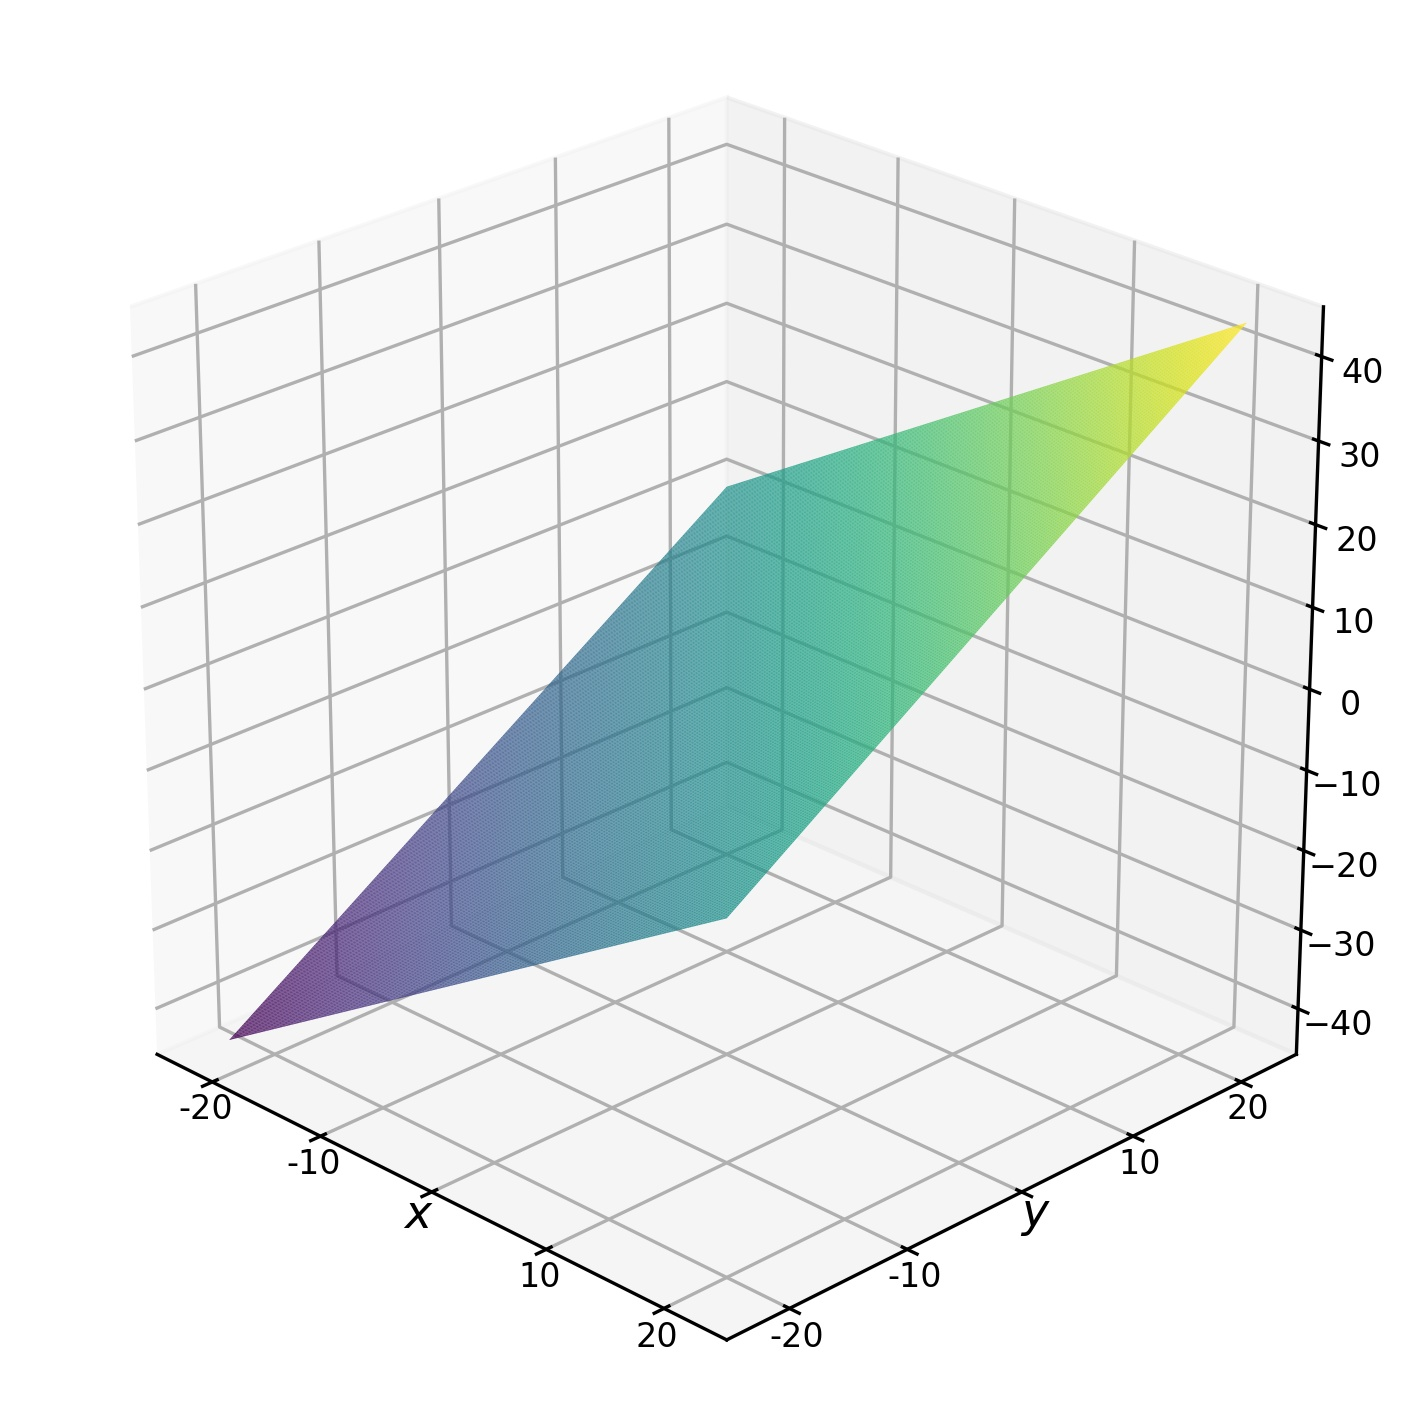
\includegraphics[
        width=.5\textwidth,
        trim=0 .55cm 0 .8cm,
        clip
    ]{funcoesRn/planoXpY.jpg}
    \caption{Gráfico da função $f(x,y)=x+y$.}
    \label{fig:planoXpY}
\end{figure}
\begin{example}\label{exemplo:paraboloide}
    Seja $f:\mathbb R^2\to\mathbb R$ dada por
    \[
        f(x,y)=x^2+y^2.
    \]
    Então
    \[
        \operatorname{Graf}(f)
        =
        \{(x,y,z)\in\mathbb R^3:z=x^2+y^2\}.
    \]
    Nesse caso, o valor de $f(x,y)$ é sempre não negativo.
    Além disso, quanto mais distante $(x,y)$ está da origem do plano, maior é a altura $z=x^2+y^2$.

    O gráfico é uma superfície em formato de paraboloide, com ponto mais baixo em $(0,0,0)$.
    As seções horizontais do gráfico obtidas fixando $z=c$, com $c>0$, são
    \[
        \{(x,y,c)\in\mathbb R^3:x^2+y^2=c\},
    \]
    isto é, circunferências de raio $\sqrt c$ no plano $z=c$.

    O gráfico desse paraboloide pode ser visualizado na Figura~\ref{fig:paraboloide}.
\end{example}
\begin{figure}[ht]
    \centering
    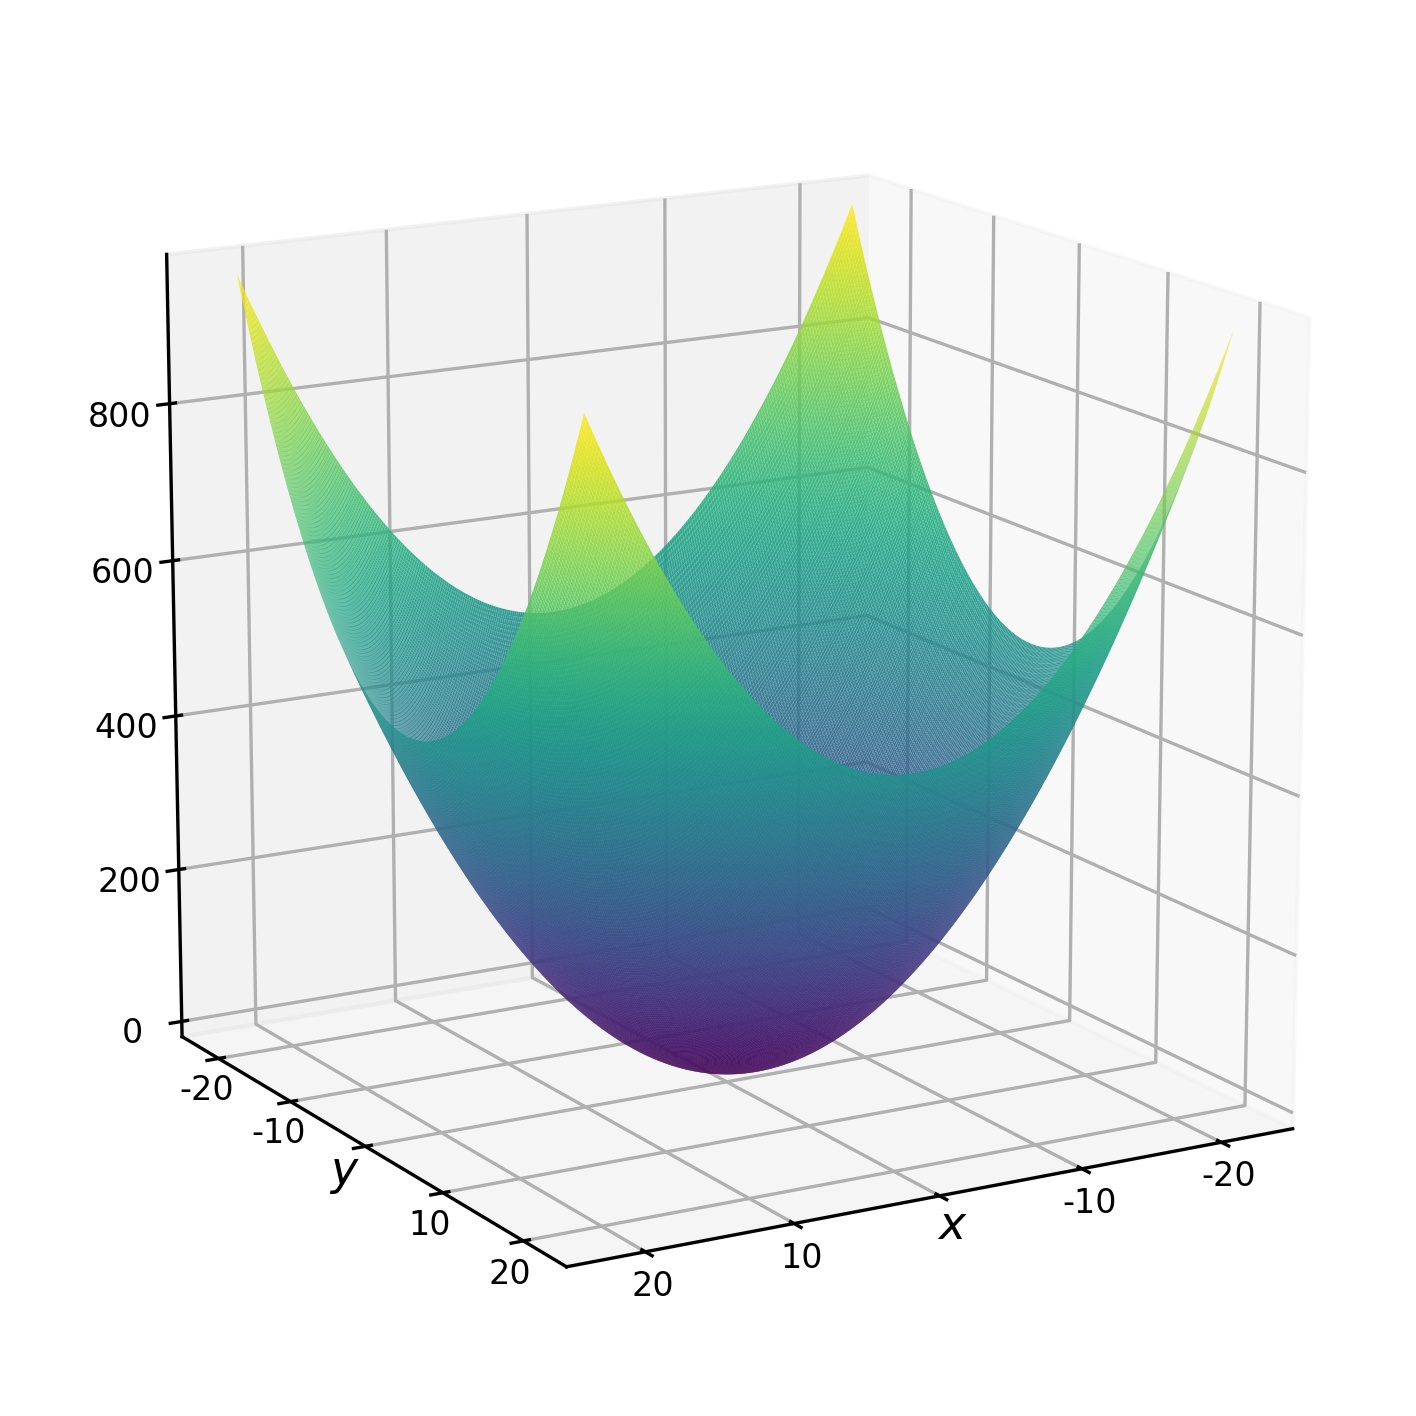
\includegraphics[
        width=.5\textwidth,
        trim=0 0.95cm 0 1.50cm,
        clip
    ]{funcoesRn/paraboloide.jpg}
    \caption{Gráfico da função $f(x,y)=x^2+y^2$.}
    \label{fig:paraboloide}
\end{figure}

\subsection*{Exercícios}

\begin{exercise}
    Seja $f:\mathbb R\to\mathbb R^4$ dada por
    \[
        f(t)=(t^2,\, t-1,\, 3,\, 2t+1).
    \]
    Determine as funções coordenadas $f_1,f_2,f_3,f_4:\mathbb R\to\mathbb R$.
\end{exercise}

\begin{exercise}
    Sejam $f,g:\mathbb R^2\to\mathbb R^2$ dadas por
    \[
        f(x,y)=(x+y,x-y)
        \qquad\text{e}\qquad
        g(x,y)=(x^2,y^2).
    \]
    Determine as expressões das funções $f+g$, $f-g$, $2f$ e $f\cdot g$.
\end{exercise}

\begin{exercise}
    Sejam $f,g:\mathbb R^2\to\mathbb R$ dadas por
    \[
        f(x,y)=x+y
        \qquad\text{e}\qquad
        g(x,y)=x-y.
    \]
    Determine o domínio e a expressão das funções $\dfrac{1}{f}$, $\frac{1}{g}$, $\frac{f}{g}$ e $\frac{g}{f}$.
\end{exercise}

\begin{exercise}
    Seja $D=\{(x,y)\in\mathbb R^2:x^2+y^2\leq 1\}$ e seja $f:D\to\mathbb R$ dada por
    \[
        f(x,y)=0.
    \]
    Descreva explicitamente o gráfico de $f$ como subconjunto de $\mathbb R^3$.
    Interprete geometricamente esse gráfico.
\end{exercise}

\begin{exercise}
    Seja $f:\mathbb R^2\to\mathbb R$ dada por
    \[
        f(x,y)=x^2+y^2.
    \]
    Determine a interseção de $\operatorname{Graf}(f)$ com o plano horizontal $z=4$.
    Interprete geometricamente essa interseção.
\end{exercise}